% 03-method.tex — truth: 本文件（2026-11-15 深度改造: R3-2/R3-3/R2-4 落实）
%   R3-2: A/P 显式区分 + Eq.(4) 组(原型=类均值、共识门、m_c 频率缩放);
%   R3-3: 种子=高召回低精度先验, 验证流程与标注成本单列, 预算核算口径统一;
%   R2-4: m_c 在 Eq. 组后给最小定义, 完整形式声明见补充材料;
%   AimCLR→SMQ 接口说明入 §3.2.2; SMQ 降级为辅助步骤。
% 纪律: galaxy Method 规范——呈现设计决策, 验证数字留 §4(E1-E6 各段), 此处不重复 Evidence 块;
% fig2 落 §3.3(规格 figure-specs.md, PDF 待绘); Algorithm 1 用 algorithm/algpseudocode.
\section{Method}\label{sec:method}

This section presents the Physics--Semantics Decoupled framework (PSD). Section~\ref{ssec:formulation} fixes notation and gives an overview. Section~\ref{ssec:physics} details the physics layer, which learns \emph{how skeletons move} without any behavior labels. Section~\ref{ssec:semantic} details the semantic layer, which learns \emph{what behaviors are called} from a small seed budget. Section~\ref{ssec:decoupling} formalizes the decoupling mechanism that absorbs evolving evaluation criteria.

\subsection{Problem formulation and overview}\label{ssec:formulation}

\paragraph{Notation.}
Let $X = \{x_1, \dots, x_T\}$ denote an unlabeled skeleton stream, where $x_t \in \mathbb{R}^{J \times 3}$ holds 3D joint coordinates for $J$ joints at frame $t$. A taxonomy $\mathcal{Y}$ maps behavior names to labels; evaluation criteria evolve by replacing $\mathcal{Y}$ with $\mathcal{Y}'$. The annotation budget is a set $S$ of seed clips with coarse labels produced by a rule engine over physical priors; $U$ denotes the unlabeled proposal set, $P$ the prototype set, and $B$ the human-annotation budget in clips consumed by the queue. We write $A = \{(e_i, \tilde{y}_i)\}_{i=1}^{N_A}$ for the \emph{seed anchors}---physics-layer embeddings $e_i = \Phi(s_i)$ of seed segments $s_i \in S$ carrying rule-engine coarse labels $\tilde{y}_i$---and reserve $P = \{(\mu_c, y_c)\}$ for the \emph{class prototypes}; the two are distinct objects (Section~\ref{ssec:proto}).

\paragraph{Framework overview.}
PSD factorizes recognition into two layers with a narrow interface. The \emph{physics layer} $\Phi$ maps skeleton windows to dynamics embeddings, trained once per species family on unlabeled streams; it comprises self-supervised pretraining (Section~\ref{ssec:pretrain}) and unsupervised temporal segmentation (Section~\ref{ssec:segmentation}). The \emph{semantic layer} $\Omega$ maps dynamics embeddings and segment proposals to labels under the current taxonomy $\mathcal{Y}$; it comprises seed-anchor construction (Section~\ref{ssec:anchors}), prototype clustering with iterated pseudo-labeling (Section~\ref{ssec:proto}), and semi-supervised self-training with small-budget initialization (Section~\ref{ssec:selftrain}). The layers interact only through embeddings and proposals. This constraint is what allows $\mathcal{Y} \to \mathcal{Y}'$ transitions to leave $\Phi$ untouched (Section~\ref{ssec:decoupling}).

\subsection{Physics layer}\label{ssec:physics}

\subsubsection{Self-supervised pretraining}\label{ssec:pretrain}

We adapt extreme-asymmetry contrastive pretraining~\citep{guo2022aimclr} to quadruped skeletons. Three adaptations matter. First, the joint graph is rebuilt for the target species topology rather than the human body plan; our pipeline uses a 24-joint quadruped layout mapped into an NTU-compatible view via an identity correspondence plus one dead slot. Second, augmentation primitives are restricted to transformations that preserve quadruped plausibility. Third, the official weight initialization is deliberately skipped: re-initializing all convolutional and linear weights to $\mathcal{N}(0, 0.02)$ collapses representations into a cone from which InfoNCE cannot escape on our data, and skipping it restores normal convergence. We report this as a reproducibility note for practitioners reusing official code bases.

\subsubsection{Unsupervised temporal segmentation}\label{ssec:segmentation}

Continuous skeleton streams must be cut into behavior-proposal units before labeling. We use motion-word quantization~\citep{gokay2025smq} as an \emph{auxiliary front-end}, not as a contribution claim: local motion patterns are quantized into a discrete vocabulary, and segment boundaries are proposed where the quantized sequence changes regime.

\paragraph{Interface to the physics encoder.}
SMQ consumes the same species-adapted skeleton view that the physics layer is trained on---SMAL-native 24-joint coordinates resampled to a fixed window---rather than the NTU-compatible 25-slot view used inside AimCLR; a dedicated adapter performs the view conversion, so the two components share data provenance but neither consumes the other's internal representations. On the embedding side, SMQ delivers only segment boundaries: every proposal is then encoded by the \emph{frozen} $\Phi$ into a dynamics embedding (the same features the semantic layer consumes), and no SMQ-internal codebook or quantizer state enters $\Omega$. The interface is therefore exactly ``(boundaries in, $\Phi$-embeddings out)'', which keeps the segmentation module replaceable---Section~\ref{sec:ablation} ablates SMQ against uniform-window and fixed-grid alternatives under this same interface, and reports the comparison honestly: on the small public-real evaluation suite SMQ's boundary IoU is statistically on par with a fixed-grid probe, so the segmentation choice is a measured operating decision rather than a load-bearing component of our claims.

\subsection{Semantic layer}\label{ssec:semantic}

The semantic layer grows labeled coverage toward completeness of the taxonomy from the rule-engine seed set $S$, following the anchor--cluster--pseudo-label recipe transferred from image-domain few-shot recognition~\citep{snell2017prototypical} (Section~\ref{ssec:rw-semi}).

The transfer required re-engineering, not re-application, because three domain shifts bind: First, anchors must be defined over \emph{temporal segment embeddings} from a self-supervised physics encoder instead of image features, so anchor quality depends on representation adequacy (Section~\ref{ssec:pretrain}). Second, prototype clustering operates on variable-length proposals delivered by unsupervised segmentation rather than fixed-size inputs, coupling label-expansion quality to segmentation quality (Section~\ref{ssec:segmentation}). Third, confidence calibration must tolerate quadruped kinematics whose intra-class motion variance differs from both image textures and human locomotion. Each shift is validated separately in Sections~\ref{sec:experiments}--\ref{sec:ablation} before the composed pipeline is evaluated.

\subsubsection{Seed anchors and their verification}\label{ssec:anchors}

Rule-engine coarse labels over physical priors provide seed anchors $A = \{(e_i, \tilde{y}_i)\}$, where $e_i$ are physics-layer embeddings of seed segments and $\tilde{y}_i$ are the engine's coarse labels. Anchors are the \emph{only} labeled objects the loop consumes; unlike anchor-based contrastive objectives that treat anchors as sample pairs~\citep{mac2022learning}, our anchors carry semantic identity and directly supervise cluster assignment.

\paragraph{Seeds are priors, not ground truth.}
The rule engine is deliberately tuned for high recall at the cost of precision: it triggers on physical priors (paw-height ordering for gait classes, head-cluster height for posture classes) and emits a per-segment confidence from rule margin, with short ambiguous spans merged into high-confidence neighbors. We therefore treat every seed label $\tilde{y}_i$ as a noisy prior, never as ground truth, in three concrete ways. (1)~\emph{Quality gating at ingestion}: seed segments enter $A$ only if the engine's own confidence is at least $0.8$ and the segment spans at least $0.5$\,s; segments labeled \emph{unknown} are discarded. (2)~\emph{Verification before write-back}: only seed labels that survive a human spot-check enter the verified anchor set used by the consolidation step (Section~\ref{ssec:selftrain}); unverified seeds supervise only the expansion loop, whose confidence gate is calibrated to tolerate their noise. (3)~\emph{Noise robustness by construction}: anchors initialized from noisy seeds are corrected by confidence-filtered cluster consensus and audited in downstream evaluation (Section~\ref{sec:ablation} reports the seed-noise injection study) rather than trusted as ground truth.

\paragraph{What seed verification costs.}
The verification budget is part of the annotation accounting and is never free. Concretely, verifying one seed clip means a human auditor watches the segment and confirms or corrects its coarse label---a binary decision per segment, an order of magnitude cheaper than full frame-level annotation of the same clip, which requires marking onset and offset of every behavior. Under the loop's accounting, the effective supervision budget is therefore $|S_{\mathrm{verified}}| + |S_{\mathrm{unverified}}| \cdot c_{\mathrm{spot}} + B$ clips-equivalents, where $c_{\mathrm{spot}} \ll 1$ is the per-clip spot-check cost in units of full clip annotations and $B$ is the low-confidence queue budget of Section~\ref{ssec:proto}. We report annotation units in this caliber throughout, and the seed clips consumed by the warm-start initialization of Section~\ref{ssec:selftrain} are counted inside $|S|$, not in addition to it: warm-starting reuses \emph{already-verified} source-domain anchors, so it adds no new seed cost---the remaining marginal cost of adaptation is the $B$ (or, at minimum, 20-clip) offset-domain budget, which is how the budget curves of Section~\ref{sec:experiments} are read.

\subsubsection{Prototype clustering and iterated pseudo-labeling}\label{ssec:proto}

\paragraph{Anchors versus prototypes.}
Seed anchors $A$ and class prototypes $P$ are different objects with different roles, and conflating them is precisely the confusion this subsection removes. Anchors are \emph{labeled exemplar embeddings}: a fixed set of (embedding, coarse-label) pairs produced by the rule engine, consumed as supervision, and never re-estimated. Prototypes are \emph{class-representative vectors}: one per taxonomy class under the current round's labeling state, maintained as free parameters of $\Omega$ and re-estimated every round. A prototype is always the \emph{class mean} of the labeled support it represents: given the currently labeled set (verified seeds plus the confidence-filtered pseudo-labeled pool), the prototype of class $c$ is
\begin{equation}\label{eq:proto}
\mu_c \;=\; \frac{\sum_{i \in \mathcal{I}_c} \phi(e_i)}{\bigl\lVert \sum_{i \in \mathcal{I}_c} \phi(e_i) \bigr\rVert_2}, \qquad \mathcal{I}_c = \{\, i : \text{$i$ labeled as $c$ in the current round} \,\},
\end{equation}
where $\phi(\cdot)$ denotes $\ell_2$ normalization; i.e., the mean of the support members' normalized embeddings, re-normalized. Initially $\mathcal{I}_c$ contains only seed anchors with $\tilde{y}_i = c$; as pseudo-labels accumulate, pool members join $\mathcal{I}_c$ and $\mu_c$ tracks the class mean of the union. This update rule is deliberately the plain class mean---no momentum, no learned projection---so that prototype drift is fully attributable to the labeled-set composition, which the stopping rule of Algorithm~\ref{alg:pseudoloop} monitors.

\paragraph{Assignment, consensus, and admission.}
Unlabeled proposals from Section~\ref{ssec:segmentation} are embedded by $\Phi$ and assigned by the current classifier $\Omega$ (the \emph{head path}); the prototype path provides a second opinion. Writing $\hat{y}_u^{\Omega}$ for the head's prediction, $p^{(1)}_u \geq p^{(2)}_u$ for its top-1 and top-2 class posteriors, and $\hat{y}_u^{P}$ for the nearest-prototype prediction $\arg\max_c \phi(\Phi(u))^{\top} \mu_c$, a proposal $u$ is admitted to the pseudo-label pool only if
\begin{equation}\label{eq:pool}
\underbrace{\hat{y}_u^{\Omega} = \hat{y}_u^{P}}_{\text{prototype consensus}} \;\wedge\; \underbrace{\kappa(u) \,\geq\, \tau_{\hat{y}_u^{\Omega}}}_{\text{calibrated margin gate}}, \qquad \kappa(u) = \frac{p^{(1)}_u - p^{(2)}_u}{m_{\hat{y}_u^{\Omega}}},
\end{equation}
where $\kappa(u)$ is the calibrated top1$-$top2 margin. The consensus condition is governed by the designated high-error seed class in the physics-prior label space (the standing posture in our instantiation); on tiers whose taxonomy lacks that class it degenerates to the margin gate alone, and nearest-prototype assignment is the ablated fallback configuration. Proposals passing Eq.~\eqref{eq:pool} receive pseudo-labels; the pool is re-filtered each round (replacement, not monotone accumulation); prototypes are then re-estimated by Eq.~\eqref{eq:proto}. Figure~\ref{fig:pseudoloop} depicts the loop and Algorithm~\ref{alg:pseudoloop} summarizes it.

\paragraph{Class-specific thresholds and $m_c$.}
The operating threshold $\tau$ is fixed once by quantile targeting on estimated coverage at the first round (the same $\tau$ is reused in every later round to prevent drift), and each class receives a scaled threshold
\begin{equation}\label{eq:mc}
\tau_c \;=\; \tau \cdot m_c, \qquad m_c = f\!\left(\pi_c / \pi_{\max}\right),
\end{equation}
where $m_c$ is a \emph{frequency-aware scaling factor} built from the ratio of class $c$'s seed prior $\pi_c$ to the largest class prior $\pi_{\max}$: rare classes receive $m_c \leq 1$ (a lower admission bar, countering long-tail suppression), majority classes receive $m_c \approx 1$, and a floor prevents the bar from collapsing on extreme tails. The concrete functional form of $f(\cdot)$ and its sensitivity parameters (exponent and floor ratio) are hyperparameters of the protocol rather than tuned per benchmark; we state the required shape here and give the exact instantiation, default values, and ablation hooks in the supplementary material.

\begin{figure}[pos=tbp]
  \centering
  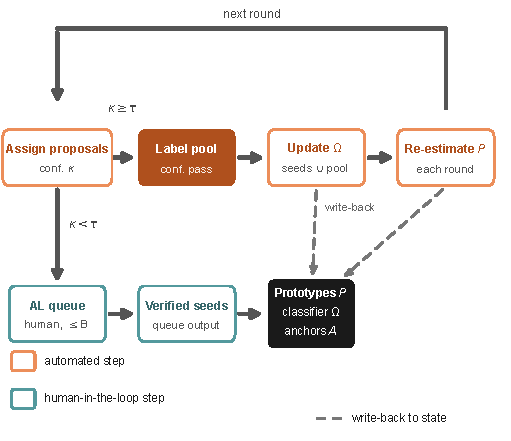
\includegraphics[width=\linewidth]{fig2_pseudo_label_loop.pdf}
  \caption{The anchor-guided pseudo-labeling loop as a two-row pipeline around a shared state hub. Automated loop (top row, left to right): Assign proposals applies the consensus-and-margin gate of Eq.~\eqref{eq:pool} ($\hat{y}^{\Omega}_u = \hat{y}^{P}_u$ and $\kappa(u) \geq \tau_{\hat{y}^{\Omega}_u}$) to route admitted proposals into the label pool; $\Omega$ is updated on verified seeds $\cup$ pool, prototypes are re-estimated by the class-mean update of Eq.~\eqref{eq:proto}, and the next round returns to Assign along the top. Human branch (bottom row): low-confidence proposals ($\kappa < \tau$) divert to an annotation queue (budget $B$ of 100--200 clips); verified seeds write back to the anchor set $A$. The dark hub carries the shared state ($P$, $\Omega$, $A$) that the dashed write-back spokes update each pass; the physics encoder $\Phi$ remains frozen throughout (not shown). Orange-labeled steps are automated; teal-labeled steps are human-in-the-loop. The annotation queue is a deployment extension of Algorithm~\ref{alg:pseudoloop}.}\label{fig:pseudoloop}
\end{figure}

\begin{algorithm}[t]
\caption{Anchor-guided iterative pseudo-labeling}\label{alg:pseudoloop}
\begin{algorithmic}[1]
\Require physics encoder $\Phi$ (frozen), seed anchors $A$, unlabeled proposals $U$, threshold $\tau$, margins $m_c$
\Ensure classifier $\Omega$ under taxonomy $\mathcal{Y}$
\State initialize prototypes $P$ as class means of $A$ (Eq.~\eqref{eq:proto})
\Repeat
  \State assign each $u \in U$ via $\Omega$; prototype opinion $\hat{y}^{P}_u$; confidence $\kappa(u)$
  \State $L_{\mathrm{high}} \leftarrow \{u : \hat{y}^{\Omega}_u = \hat{y}^{P}_u \wedge \kappa(u) \geq \tau_{\hat{y}^{\Omega}_u}\}$ (Eq.~\eqref{eq:pool}); re-filter the pseudo-labeled pool (replacement)
  \State update $\Omega$ on verified seeds $\cup$ pseudo-labeled pool
  \State re-estimate $P$ as class means of the labeled set (Eq.~\eqref{eq:proto})
\Until{proposal assignment stabilizes, the iteration budget is reached, or (where a rule-derived consensus reference exists) pool precision against it drops for two consecutive rounds}
\end{algorithmic}
\end{algorithm}

Design decisions fixed at this stage: confidence filtering uses calibrated classifier margins divided by the class margin scale $m_c$ (prototype margins in the fallback path); each iteration retrains only $\Omega$, never $\Phi$; the iteration budget guards against confirmation bias accumulating across rounds; and seed-noise amplification is bounded by the three-part seed treatment of Section~\ref{ssec:anchors} (ingestion gating, spot-check verification before write-back, and consensus correction), so rule-engine seeds act as high-recall/low-precision priors rather than ground truth. The precision-drop stopping rule monitors pool precision against the physics-prior consensus reference---a weak, rule-derived proxy rather than human annotation. On tiers where training-split labels are fully observed but no rule-derived consensus exists (the Animal Kingdom and NTU end-to-end arms), the rule is disabled and iteration stops on convergence or the iteration budget; the consolidated classifier consumes verified seed labels plus pseudo-labels for pool clips, never pool ground truth. Class imbalance in animal behavior distributions (long-tail rare behaviors) is handled at the prototype level via the frequency-aware thresholds of Eq.~\eqref{eq:mc} rather than resampling; a head-to-head ablation of this choice (margins vs.\ resampling vs.\ no handling) is registered for the public-real tier and not yet run (Section~\ref{sec:ablation}, Sensitivity). The consensus condition of Eq.~\eqref{eq:pool} governs a designated high-error seed class (the standing posture in the physics-prior label space); on tiers whose taxonomy lacks that class (the Animal Kingdom and NTU class spaces) it passes all proposals by construction.

\subsubsection{Semi-supervised self-training and small-budget initialization}\label{ssec:selftrain}

Pseudo-labeled coverage is consolidated by iterative retraining of $\Omega$ on the growing pool---pool clips enter with their pseudo-labels, and only \emph{verified} seed clips contribute ground-truth labels---in the semi-supervised self-training tradition motivated by TCL~\citep{singh2021tcl} (whose temporal-contrastive consolidation step is not used here). To make very small annotation budgets usable, a warm-start protocol initializes small-budget training from the semantic-layer weights of a full-budget model trained on the same taxonomy under the noise-offset protocol of Section~\ref{sec:experiments}, before expansion proceeds within the budget $B$. Warm-starting is a transfer of \emph{verified} source-domain anchors and semantic-layer weights, so it consumes no new seed budget; the total supervision accounting (verified seeds, spot-check effort, and the target-domain budget) follows Section~\ref{ssec:anchors}. Figure~\ref{fig:pseudoloop} illustrates the complete loop.

\subsection{Decoupling mechanism}\label{ssec:decoupling}

We formalize an evaluation-criteria evolution as a taxonomy transition $\mathcal{Y} \to \mathcal{Y}'$ (splitting, merging, renaming, or adding behaviors). We report the transition cost $C(\mathcal{Y} \to \mathcal{Y}')$ as a pair---human annotation units consumed and wall-clock retraining time---kept in separate units rather than summed, measured at matched final accuracy. Under decoupling: (1) the physics layer $\Phi$ and its pretrained parameters remain frozen; (2) existing segment proposals are re-used---only their label assignments change; (3) the semantic layer is rebuilt through Section~\ref{ssec:semantic} using seeds under $\mathcal{Y}'$; and (4) the reported quantity is $C_{\mathrm{decoupled}}(\mathcal{Y} \to \mathcal{Y}')$ versus $C_{\mathrm{full}}(\mathcal{Y} \to \mathcal{Y}')$, where the full baseline retrains representation learning under $\mathcal{Y}'$. We hypothesize that $C_{\mathrm{decoupled}} < C_{\mathrm{full}}$ at matched accuracy, and that accuracy under $\mathcal{Y}'$ matches full retraining within noise; Section~\ref{sec:experiments} (E6) tests both hypotheses.
